\documentclass[a4paper,12pt]{article}
\usepackage{jae}
\usepackage{amsmath, bm, amsfonts}

\title{Spatial models for distance sampling data: recent developments and future directions}
\running{Spatial models for distance sampling}

\author{
David L. Miller$^{1*}$, \and
M. Louise Burt$^{2}$, \and
Eric A. Rexstad$^{2}$, \and 
Len Thomas$^{2}$.}

\affiliations{
\item Department of Natural Resources Science, University of Rhode Island, Kingston, Rhode Island 02881, USA
\item Centre for Research into Ecological and Environmental Modelling,\\ The Observatory, University of St. Andrews, St. Andrews KY16 9LZ, UK
}
\nwords{4309}
\ntables{0}
\nfig{5}
\nref{31}

\corr{\url{dave@ninepointeightone.net}}

\begin{document}

\maketitle

\begin{abstract}
  \noindent 

\begin{enumerate}
	\item Our understanding of a biological population can be greatly enhanced by modelling their distribution in space and as a function of environmental covariates. 
	\item Density surface models consist of a spatial model of the abundance of a biological population which has been corrected for uncertain detection via distance sampling methods. 
	\item We offer a comparison of recent advances in the field and consider the likely directions of future research. In particular we consider spatial modelling techniques that may be advantageous to applied ecologists such as quantification of uncertainty in a two-stage model and smoothing in areas with complex boundaries.
	\item The methods discussed are available in an \textsf{R} package developed by the authors and are largely implemented in the popular Windows package Distance (or are soon to be incorporated).
	\item Density surface modelling enables applied ecologists to reliably estimate abundances and create maps of animal/plant distribution. Such models can also be used to investigate the relationships between distribution and environmental covariates.
\end{enumerate}
 

\end{abstract}

\noindent \textbf{Keywords:} abundance estimation, Distance software, generalized additive models, line transect sampling, point transect sampling, population density, spatial modelling, wildlife surveys


\newpage

\section*{Introduction}
\label{s:intro}

When surveying biological populations it is increasingly common to record spatially referenced data, for example: coordinates of observations, habitat type, elevation or (if at sea) bathymetry. Spatial models allow for vast databases of spatially-referenced data \citep[e.g. OBIS-SEAMAP,][]{Halpin:2009je} to be harnessed, enabling investigation of interactions between environmental covariates and population densities. Mapping the spatial distribution of a population can be extremely useful, especially when communicating results to non-experts. Recent advances in both methodology and software have made spatial modelling readily available to the non-specialist \citep[e.g.,][]{Wood:2006wz, Rue:2009tw}. Here we use the term ``spatial model'' to include any model that includes spatially referenced covariates, not just smooths of location. This article is concerned with combining spatial modelling techniques with distance sampling \citep{Buckland:2001vm, Buckland:2004ts}. 

Distance sampling takes plot sampling (counting all the individuals or groups of objects within a strip or circle) and extends it to the case where detection is not certain. Observers move along lines or stand at points and record the distance from the  line or point to the object of interest ($y$). These distances are used to estimate the \textit{detection function}, $g(y)$ (Fig. \ref{dolphin-df}), by modelling the decrease in detectability with increasing distance from the line or point (conventional distance sampling, CDS). The detection function may also include covariates \citep[multiple covariate distance sampling, MCDS;][]{Marques:2007vm} which affect the scale of the detection function. From the fitted detection function, the probability of detection can be estimated. The estimated probability that an animal is detected, $\hat{p}_i$, can then be used to estimate abundance as

\begin{equation}
\hat{N} = \frac{A}{a} \sum_{i=1}^{n} \frac{1}{\hat{p}_i},
\label{ht-est}
\end{equation}
where $A$ is the area of the study region, $a$ is the area covered by the survey (i.e., the sum of the areas of all of the strips/circles) and the summation takes place over the $n$ observed individuals \citep[Chapter 3]{Buckland:2001vm}. In general distance sampling is more efficient than plot sampling because a much higher proportion of observations can be used in the analysis. Often up to half the observations in a plot sampling data set are discarded to ensure the assumption of certain detection is met. In contrast, distance sampling uses the observations that would have been discarded to model the detection (typically data are discarded beyond a given \textit{truncation distance} during analysis).

When fitting the detection function in a distance sampling analysis, one assumes that the objects of interest are distributed according to some process \citep[Section 2.1]{Buckland:2001vm}. It is usually possible to design surveys such that a homogenous process can be assumed so that (with respect to the line) objects are distributed uniformly. This can be achieved by ensuring that  transects randomly located.

Estimators such as eqn (\ref{ht-est}) rely on the design of the study to ensure that abundance estimates over the whole study area (scaling up from the covered region) are valid. By contract this article focusses on \textit{model-based} inference to extrapolate to a larger study area. Specifically, we consider the use spatially explicit models to investigate the response of biological populations to biotic and abiotic covariates that vary over the study region. A spatially-explicit model can explain the between transect variation (which is often a large component of the variance in design-based estimates) and so using a model-based approach can lead to smaller variance in estimates of abundance. Model-based inference also enables the use of data from opportunistic surveys, for example, incidental data arising from ``ecotourism'' cruises \citep{Williams:2006tz}. 

Our aims in creating a spatial model of a biological population are usually two-fold: (i) estimating overall abundance and (ii) investigating the relationship between abundance and environmental covariates. As with any predictions that are outside the range of the data, one should heed the usual warnings regarding extrapolation. For example, if a model contains elevation as a covariate, predictions at high, unsampled elevations are unlikely to be reliable. Frequently, maps of abundance or density are required and any spurious predictions can be visually assessed, as well as by plotting a histogram of the predicted values. A sensible definition of the region of interest avoids prediction outside the range of the data.

In this article we review the current landscape of spatial modelling of distance sampling data, illustrating some recent developments most useful to applied ecologists. The methods discussed have available in the popular Windows application Distance \citep{Thomas:2010cf} for some time but the recent advances covered here have been implemented in a new \textsf{R} package, \texttt{dsm} \citep{dsm-package}  and are soon to incorporated into Distance.

Throughout this article a motivating data set is used to illustrate the methods. These data are from a combination of several shipboard surveys conducted on several cetacean species in the Gulf of Mexico. We investigate 47 observations of groups of pantropical spotted dolphins (\textit{Stenella attenuata}); group size was recorded, as well as the Beaufort sea state at the time of the observation. Coordinates for each observation and bathymetry data were available as covariates for the analysis. A complete example analysis is provided as an online appendix. The data used in the analysis are available in the \texttt{dsm} package and Distance.

The rest of the article follows this structure: we first introduce the density surface modelling approach of \cite{Hedley:2004et}; explain how to estimate abundance and uncertainty; describe recent advances and provide practical advice regarding model fitting, formulation and checking. Before concluding, we review alternative (but less mature) methods which take a more direct approach to modelling spatial distance sampling data.


\section*{Density surface modelling}
\label{s:dsm}

This section focuses on modelling the density/abundance estimation stage of distance sampling, using the ``count model'' of \cite{Hedley:2004et}, which we refer to as \textit{density surface modelling} (DSM). Both line and point transects can be used but if lines are used then they are are split into contiguous \textit{segments} (indexed by $j$), which are of length $l_j$. Segments should be small enough such that neither density of objects or covariate values vary appreciably within a segment (usually making the segments approximately square, $2w\times 2w$, is sufficient). Count or estimated abundance is then modelled as a smooth function of covariates using a generalized additive model \cite[GAM; e.g.][]{Wood:2006wz}. For each segment or point, the response is modelled as a function of environmental covariates that are measured at the segment/point level ($z_{jk}$ with $k$ indexing the covariates, e.g., location, sea surface temperature, weather conditions). The area of each segment enters the model as (or as part of) an offset: the area of segment $j$ is $A_j = 2wl_j$ and at point $j$ is $A_j=w\pi^2$ (where $w$ is the truncation distance). 

\subsection*{Count as response}

The model for the count per segment is:

\begin{equation*}
\mathbb{E}(n_j) = \exp\left[ \log_e \left( \hat{p}_j A_j \right) + \beta_0 + \sum_k f_k\left(z_{jk}\right) \right],
\end{equation*}
where the $f_k$s are smooth functions of the covariates and $\beta_0$ is an intercept term. Multiplying the segment area ($A_j$) by the probability of detection ($\hat{p}_j$) gives the \textit{effective area} for segment $j$. If there are no covariates other than distance in the detection function then the probability of detection is constant for all objects observed in the segment (i.e., $\hat{p}_j=\hat{p}$, $\forall j$). The distribution of $n_j$ can be modelled as overdispersed Poisson, negative binomial, or Tweedie distribution (see \textit{Recent developments}, below).

Fig. \ref{dolphin-eda} shows the raw observations of the dolphin data, along with the transect lines, overlaid on the depth data. A half-normal detection function was fitted to the distances and is shown in Fig. \ref{dolphin-df}. Fig. \ref{fits-depth} shows a DSM fitted to the dolphin data. The top panel shows predictions from a model where depth was the only covariate, the bottom panel shows predictions where a (bivariate) smooth of spatial location was also included. The latter had a considerably lower GCV score (39.12 vs 48.46) so would be selected as our ``best'' model. 

As well as simply calculating abundance estimates, relationships between covariates and abundance can be illustrated via plots of marginal smooths. The effect of depth on abundance for the dolphin data can be seen in Fig. \ref{depth-gamplot}. 

\subsection*{Estimated abundance as response}

An alternative to modelling counts is to use the per-segment/circle abundance using distance sampling estimates as the response. In this case we replace $n_j$ by:

\begin{equation*}
\hat{N}_j = \sum_{r=1}^{R_j} \frac{s_{jr}}{\hat{p}_j},
\end{equation*}
where $R_j$ is the number observations in segment $j$ and $s_{jr}$ is the size of the $r^\text{th}$ group in segment $j$ (if the animals occur individually then $s_{jr}=1$, $\forall j,r$). 

The following model is then fitted:

\begin{equation*}
\mathbb{E}(\hat{N}_j) = \exp\left[ \log_e \left( A_j \right) + \beta_0 + \sum_k f_k\left(\bm{z}_{jk}\right) \right],
\end{equation*}
where $\hat{N}_j$, as with $n_j$, is assumed to follow an overdispersed Poisson, negative binomial, or Tweedie distribution (see \textit{Recent developments}, below). Note that the offset is now the area rather than effective area of the segment/point.

\subsubsection*{DSM with covariates at the observation level}

The above models consider the case where the covariates are measured at the segment/point level. Often covariates ($z_{ij}$, for individual/group $i$ and segment/point $j$) are collected on the level of observations; for example sex or group size of the observed object or identity of the observer. In this case the probability of detection is a function of the object (individual or group) level covariates $\hat{p}(z_i)$. Object level covariates can be incorporated into the model by adopting the following estimator of the per-segment abundance:

\begin{equation*}
\hat{N}_j = \sum_{r=1}^{R_j} \frac{s_{jr}}{\hat{p}(z_{rj})}.
\end{equation*}

By not including an offset, but instead dividing the count (or estimated abundance) by the area of the segment, we can also model density rather than abundance. We concentrate on abundance here, see \cite{Hedley:2004et} for further details on modelling density.

\subsection*{Prediction}

Abundance can be predicted for the each cell in a grid over the region in question and by summing predicted values over corresponding grid cells. The areas of the prediction cells must be accounted for in the predictions. Environmental covariates included in the model must be available at each prediction cell at the required resolution (using prediction grid cells that are smaller than the resolution of the spatially referenced data have no effect on abundance/density estimates).  

\subsection*{Variance estimation}

Estimating the variance of abundances calculated using a DSM is not straightforward: uncertainty from the estimated parameters of the detection function must be incorporated into the spatial model. A second consideration is that in a line transect survey, adjacent segments are likely to be correlated; failure to account for this spatial autocorrelation will lead to artificially low variance estimates and hence misleadingly narrow confidence intervals.

\cite{Hedley:2004et} describe a method of calculating the variance in the abundance estimates using a parametric bootstrap, resampling from the residuals of the fitted model. The bootstrap procedure is as follows.

Denote the fitted values for the model to be $\hat{\bm{\eta}}$. For $b=1,\ldots,B$ (where $B$ is the number of resamples required).
\begin{enumerate}
	\item Resample (with replacement) the per-segment residuals, store the values in $\mathbf{r}_{b}$.
	\item Refit the model but with the response set to $\hat{\bm{\eta}}+\mathbf{r}_{b}$ (where $\hat{\bm{\eta}}$ are the fitted values from the orginal model).
	\item Take the predicted values for the new model and store them.
\end{enumerate}
From the predicted values stored in the last step the variance originating in the spatial part of the model can be calculated. The total variance of the abundance estimate (over the whole region of interest or sub-areas) can then be found by combining the variance estimate from the bootstrap procedure with the variance of the probability of detection from the detection function model \citep[using the delta method which assumes that the two components of the variance are independent;][]{Seber:2002ti}.

The above procedure assumes that there is no correlation in space between segments, if many animals are observed in a particular segment then we might expect there to be high numbers in the adjacent segments. A moving block bootstrap \citep[MBB;][Section 8.6]{Efron:1993tv} can account for some of this spatial autocorrelation in the variance estimation. The segments are grouped together into overlapping blocks, (so if the block size is 5, block one is segments $1,\ldots,5$, block two is segments $2,\ldots,6$, and so on). Then, at step (2) above, resamples are taken of the blocks (contiguous collections of segments) rather than individual segments within the transects. Using blocks should account for some of the autocorrelation between the segments, inflating the variances accordingly. However, because the block size dictates the maximum amount of spatial autocorrelation accounted for, this may not fully account for the autocorrelation. These bootstrap procedures can also be modified to take into account detection function uncertainty by generating new distances from the fitted detection function and then re-calculating the offset by fitting a detection function to the new distances.
 
DSM uncertainty can be visualised via a plot of per-cell coefficient of variation obtained by dividing the standard error for each cell by its predicted abundance. 

\section*{Recent developments}
\label{s:recentadvances}

\subsubsection*{GAM uncertainty and variance propagation}

Rather than using a bootstrap, one can use GAM theory to construct uncertainty estimates for DSM abundance estimates. This requires that we use the distribution of the parameters in the GAM to simulate model coefficients, using them to generate replicate abundance estimates \citep[further information can found in][page 245]{Wood:2006wz}. Such an approach removes the need to refit the model many times, making variance estimation much faster.
 
\cite{WILLIAMS:2011in} go a step further and incorporate the uncertainty in the estimation of the detection function into the variance of the spatial model, albeit only when only segment level covariates are in the DSM. Their procedure is as follows:
\begin{enumerate}
\item Fit a density surface model.
\item Re-fit the model with an additional term that characterises the uncertainty in the estimation of the detection function (via the derivatives of the probability of detection, $\hat{p}$).
\item Variance estimates of the abundance calculated using standard GAM theory will include uncertainty from the estimation of the detection function.
\end{enumerate}
A more complete mathematical explanation of this result is given in Appendix B.

We consider that propagating the uncertainty in this manner is not only more computationally efficient but also preferable to the moving block bootstrap from a technical perspective. A moving block bootstrap does not fully account for spatial autocorrelation as when it reallocates  blocks of residuals, it does so without considering the dependence between blocks. This can then lead to wide confidence intervals. The confidence intervals produced via variance propagation are narrower than their bootstrap equivalents, while maintaining good coverage (results of a small simulation study are given in Appendix C).

Fig. \ref{cv-plot} shows a map of the coefficient of variation for the model which includes both location and depth covariates. Variance has been calculated using the variance propagation method. 

\subsection*{Edge effects}
\label{s:leakage}

Recent work \citep{Ramsay:2002uo,Wang:2007tf,Wood:2008vo,ScottHayward:2011tc,Miller:2012tm} has highlighted the need to take care when smoothing over areas with complicated boundaries, e.g., those with rivers, peninsulae or islands. If two parts of the domain (either side of a river or inlet, say) are inappropriately linked by the model (the distance between the points is measured as a straight line, rather taking into account obstacles) then the boundary feature can be ``smoothed across'' leading to incorrect inference. Ensuring that a realistic spatial model has been fitted to the data is essential for valid inference. The soap film smoother of \cite{Wood:2008vo} is appealing as the model jointly estimates boundary conditions for a complex study area along with the interior smooth. This can be helpful when uncertainty is estimated via a bootstrap as the model helps avoid large, unrealistic predictions which can plague other smoothers \citep{Bravington:2009vo}.

Even if the study area does not have a complicated boundary, edge effects can still be problematic. \cite{Miller:wx} show that global smoothers which have unpenalized plane components tend to cause the fitted surface to increase unrealistically as predictions move further away from the locations of survey effort. They suggest the use of Duchon splines (a generalisation of thin plate regression splines) to alleviate the problem.

\subsection*{Tweedie distribution}
\label{s:Tweedie}

The Tweedie distribution offers a flexible alternative to the quasi-Poisson and negative binomial distributions as a response distribution when modelling count data \citep{Candy:2004tb}. Through the parameter $\lambda$, many common distributions arise; varying $\lambda$ between 1 (Poisson) and 2 (gamma) leads to a random variable which is a sum of $M$ gamma variables where $M$ is Poisson distributed \citep{Jorgensen:1987vg}. The distribution does not change appreciably when $\lambda$ is changed by less than $0.1$ therefore, a simple line search over the possible values of $\lambda$ is usually reasonable. Mark Bravington (pers. comm.) suggested plotting the square root of the absolute value of the residuals against fitted values; a ``flat'' plot (points forming a horizontal line) give an indication of a ``good'' value for $\lambda$. We additionally suggest using the metrics described in the next section for model selection.


\section*{Practical advice}
\label{s:practical}

Fig. \ref{flow} shows a flow diagram of the modelling process for creating a DSM. The diagram shows which methods are compatible with each other and what the options are for modelling a particular data set.

In our experience, it is sensible obtain a detection function that fits the data as well as possible and only after a satisfactory detection function has been obtained, begin spatial modelling. Model selection can be performed for the detection function using AIC and model checking using goodness-of-fit tests given in \cite[Section 11.11]{burnham:2004vd}.  If animals occur in groups rather than individually, bias can be incurred due to the higher visibility of larger groups. It may then be necessary to include size as a covariate in the detection function \citep[see][Section 4.8.2.4]{Buckland:2001vm}.

Smooth terms can be selected using (approximate) $p$-values in GAM. A useful technique for covariate selection is to use an additional penalty for each term in the GAM allowing smooth terms to be removed from the model during fitting \citep[illustrated in the example analysis;][]{Wood:ub}. Smoothness selection is performed by generalized cross validation (GCV) score, UnBiased Risk Estimator (UBRE) or REstricted Maximum Likelihood (REML) score. When model covariates are effectively functions of one another (e.g. depth could be written as a function of location) GCV and UBRE can suffer from concurvity issues  which lead to failures in optimisation \cite[][Section 4.5.3]{Wood:2006wz}. The minima in GCV/UBRE tend to have less pronounced minima than REML so an optimal degree of smoothing may not be found, this can lead to unstable models \citep[slight changes in smoothness lead to vastly different results;][]{Wood:ub}. To avoid these issues REML is recommended for smoothness selection, when many spatially-referenced covariates are used. A significant drawback is that REML scores can only be used to compare models with the same fixed effects \citep[i.e. linear terms;][]{Wood:ub}. We highly recommend the use of standard GAM diagnostic plots. \cite{Wood:2006wz} provides further practical information on GAM model selection and fitting.

In the analysis of the dolphin data, we included a smooth of location. This not only nearly doubles the percentage deviance explained (27.3\% to 52.7\%), it also allows us to account for spatial autocorrelation (in a primitive way). One can see this when comparing the two plots in Fig. \ref{fits-depth} and the plot of the depth in Fig. \ref{dolphin-eda} the plot of the smooth of depth alone looks very similar to the raw plot of the depth data. A smooth of an environment-level covariate such as depth can be very useful for assessing the relationships between abundance and the covariate (as in Fig. \ref{fits-depth}). Caution should be employed when interpreting smooth relationships and abundance estimates, especially if there are gaps over the range of covariate values. Large counts may occur at a high value of depth but if no further observations occur at such a high value, then investigators should be skeptical of any relationship. A smooth of location can be useful although limiting the ``wigglyness'' of smooths of spatial location (by limiting their basis size) can be a useful way of restricting their influence whilst still allowing them to ``mop up'' the residual spatial correlation in the data (see the example analysis).


%depth only
%R-sq.(adj)                           : 0.0554 
%Deviance explained                   : 27.3%
%GCV score                          : 64.713
%
%xy + depth
%R-sq.(adj)                           : 0.292 
%Deviance explained                   : 52.7%
%GCV score                          : 52.248

In the analysis presented we have converted from latitude and longitude to kilometres from the centre of the survey region (27.01, -88.3) because the bivariate smoother used \citep[the thin plate spline;][]{Wood:2003tc} is isotropic the wigglyness of the smoother in each direction is treated equally. Moving one degree in latitude is not the same as moving one degree in longitude and so using kilometres from the centre of the study region makes the covariates isotropic (using SI units throughout would also remove the need for conversion).


\section*{Direct modelling of the spatial point process}
\label{s:direct}

Rather than use a GAM to model the spatially explicit part of the model, two recent articles \citep{Johnson:2010gf,Niemi:2010kx} have used a point process approach \citep{cox1980point}. In both cases the density of objects described by an intensity function, which can include spatially-referenced covariates.

\cite{Johnson:2010gf} propose a point process-based model for distance sampling data. They first assumed that the locations of all individuals in the survey area (not just those observed) form a realisation of a Poisson process. Parameters of the intensity function are then estimated via standard maximum likelihood methods for point processes \citep{Baddeley:2000to}. In contrast to \cite{Hedley:2004et}, all parameters are estimated jointly so uncertainty from both the spatial pattern and the detection function is incorporated into variance estimates for the abundance. This also ensures that correlations between the detection function and underlying point process are estimated correctly (and do not falsely inflate or deflate variance estimates). The authors also addressed the issue of overdispersion unmodelled by spatial covariates (i.e. counts that do not follow a Poisson mean-variance relationship) using a post-hoc correction factor.

\cite{Niemi:2010kx} also used Poisson processes but incorporate them into a fully Bayesian approach. Model fitting proceeds in two stages: first the detection function is fitted, then the spatial model (via MCMC) assuming the detection function parameters are known, so detection function uncertainty is not incorporated in the spatial model (an extension that incorporates uncertainty is, however, feasible).

Both of the above Poisson process models do not account for group size, but both state that this could be included by considering a marked point process \citep[Section 5.5]{cox1980point}. Both methods offer direct modelling of the point process, although with some drawbacks compared to the methodology of \cite{Hedley:2004et}. It should be noted that the loss of efficiency from using DSM is not large \citep[p. 313]{Buckland:2004ts} because distances contain little information about spatial variation due to the width of the transects relative to their lengths and how small circles are compared to the study area.

A final example of direct modelling of density is given in \cite{Royle:2004tu}. The authors formulate an unconditional likelihood per-point/line, which is a function of the unobserved transect abundances. These unobserved abundances are treated as (Poisson or negative binomial) random effects, which are then integrated out to give a per-transect likelihood which is a function only of detection function parameters and parameters of the random effects (linear functions of the environmental covariates). Due to the multinomial nature of the per-transect likelihood proposed distance data must be binned, resulting in a loss of information. Although an arbitrarily large number of bins could be used as an approximation, this is potentially computationally intensive.


\section*{Discussion}
\label{s:discussion}

The use of model-based inference for determining abundance and spatial distribution from distance sampling data presents new opportunities in the field of population assessment.   Inference from a sample of sightings to a population in a study area does not depend upon a random sample design, and therefore data from "platforms of opportunity" \citep{Williams:2006tz} can be used.

Unbiased estimates are dependent upon either (i) distribution of sampling effort being random throughout the study area (for design-based inference) or (ii) model correctness (for model-based inference).  It is easier to have confidence in the former than in the latter because our models are always wrong. Nevertheless model-based inference will play an increasing role in population assessment as the availability of spatially-referenced data increases.

The field is quickly evolving to allow modelling of more complex data building on the basic ideas of density surface modelling. We expect to see large advances in two areas: temporal inferences and the handling of spatial correlation. These should become more mainstream as modern spatio-temporal modelling techniques are adopted. \cite{Petersen:2011vy} provided a very basic framework for temporal modelling; their model included smooth terms both before and after the construction of an offshore windfarm. Spatial autocorrelation can be accounted for via approaches that explicitly introduce correlations such as generalized estimating equations \cite[GEEs;][]{Hardin:2003uf} or via mechanisms such as that of \cite{Skaug:2006gs}, which allowed observations to cluster according to one of several states (e.g. ``feeding'' or ``transit'') taking into account short-term agglomerations (``hot spots''). These advances should assist both modellers and wildlife managers to make optimal conservation decisions. 

Recent advances in Bayesian computation (INLA; Rue et al, 2009), make a one-step, Bayesian, density surface models computationally feasible (as INLA is an alternative to MCMC). We anticipate that such a direct modelling technique will dominate future developments in the field.

Density surface modelling allows wildlife managers to make best use of the available spatial data to understand patterns of abundance, and hence make better conservation decisions (e.g., about reserve placement). The recent advances mentioned here increase the reliability of the outputs from a modelling exercise, and hence the efficacy of these decisions.  Density surface modelling from survey data is an active area of research, and we look forward to further improvements and extensions in the near future.

\section*{Acknowledgments}

DLM wishes to thank Mark Bravington and Sharon Hedley for their help and patience in explaining and providing code for their variance propagation method. Funding for the implementation of the recent advances into the \texttt{dsm} package and Distance software came from the US Navy, Chief of Naval Operations (Code N45), grant number N00244-10-1-0057.

\newpage

\bibliography{dsm-refs}


\newpage


\newpage


\section*{Figures}

\begin{figure}[h!]
  \caption{The survey area for the example dolphin analysis, transect centrelines and observations with size of circle corresponding to the group size overlaid onto depth data.}
  \label{dolphin-eda}
  \begin{center}
    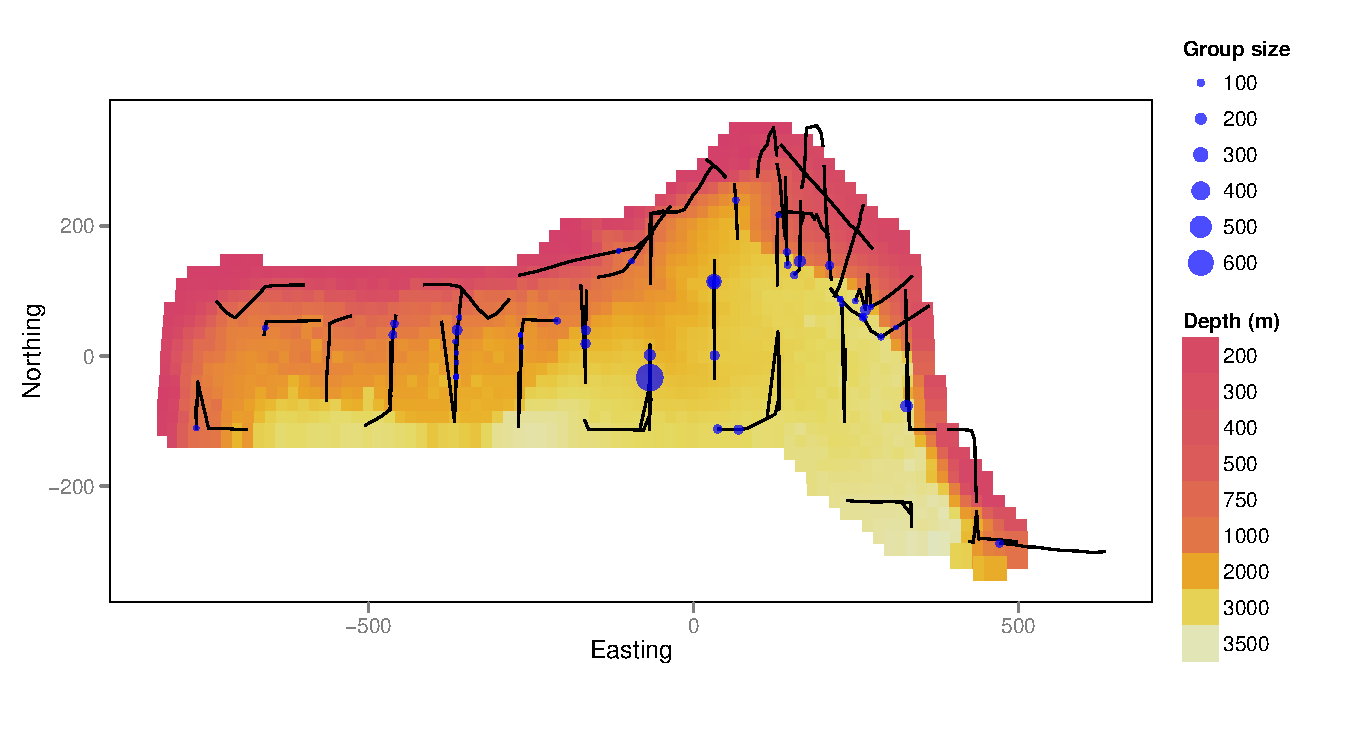
\includegraphics[width=\textwidth]{figs/depth-transects}
  \end{center}
\end{figure}

\newpage

\begin{figure}[h!]
  \caption{Histogram of observed distances with detection function fitted to the dolphin data.}
  \label{dolphin-df}
  \begin{center}
    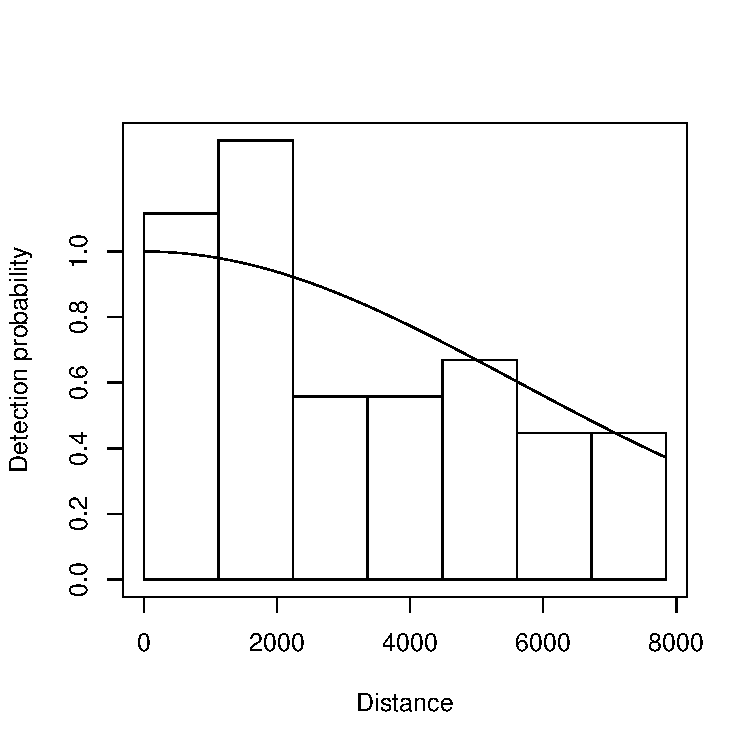
\includegraphics[width=\textwidth]{figs/distances}
  \end{center}
\end{figure}

\newpage

\begin{figure}[h!]
  \caption{Predictions for the dolphin data. Top: Predictions from the model using only depth as an explanatory variable, bottom: the model using both depth and location.}
  \label{fits-depth}
  \begin{center}
    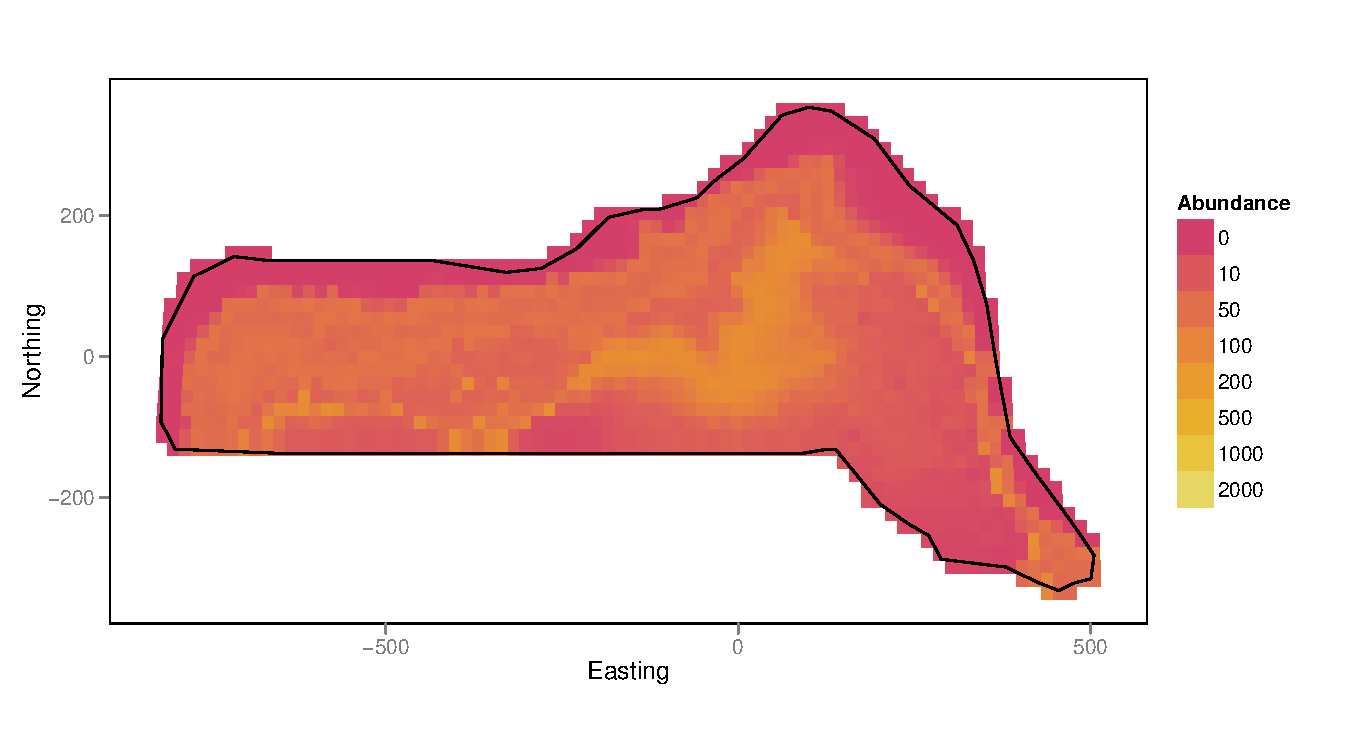
\includegraphics[width=\textwidth]{figs/fit-depth}\\
    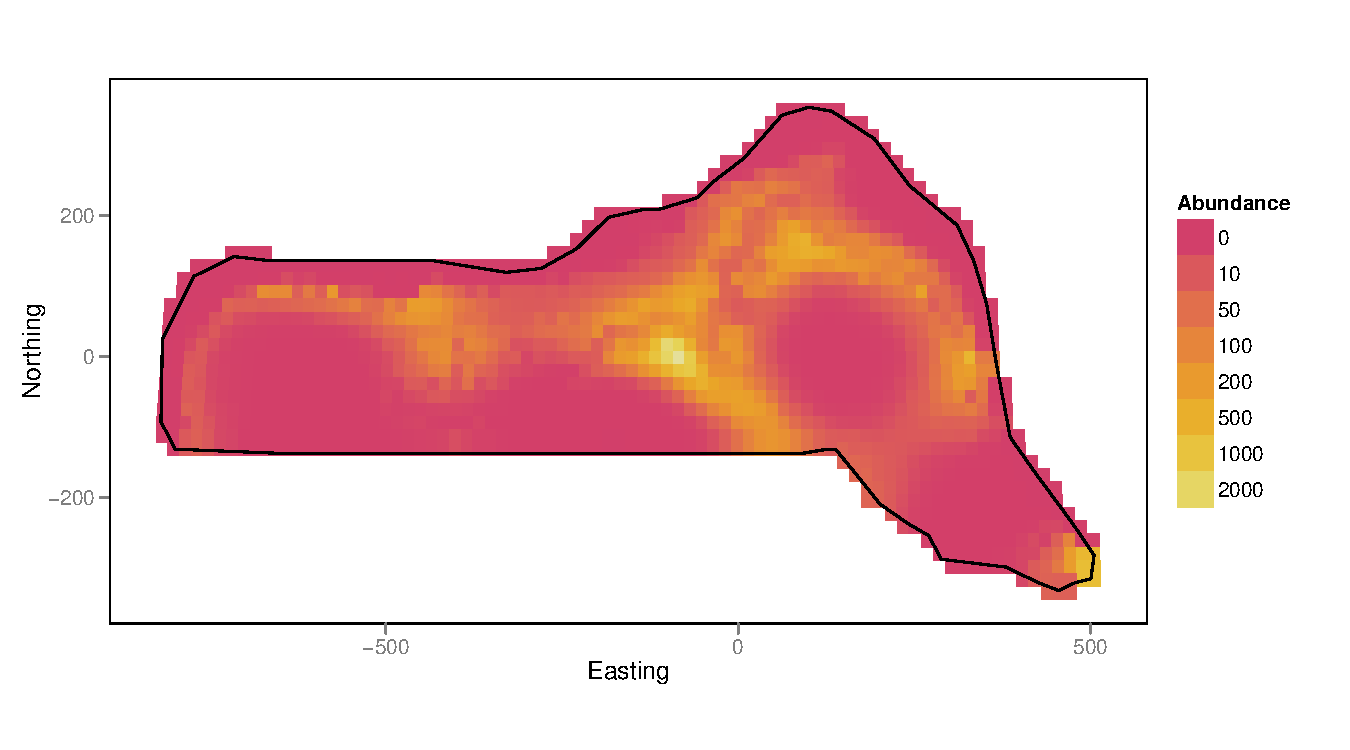
\includegraphics[width=\textwidth]{figs/fit-depth-xy}
  \end{center}
\end{figure}

\newpage

\begin{figure}[h!]
  \caption{Plot of the effect on the response of depth (from the model with both depth and location smooths), note that it is possible to draw a straight line between 750m and 3000m within the confidence band (between the dashed lines), so the wiggles in the smooth may not be indicative of any relationship. What is clear is that there is some effect up to about 500m. The rug ticks at the bottom of the plot indicate we have good coverage of the range of depth values in the survey area. Note that the $y$ axis in such plots is on the scale of the link function ($\log$ in this case), so care should be taken in their interpretation.}
  \label{depth-gamplot}
  \begin{center}
    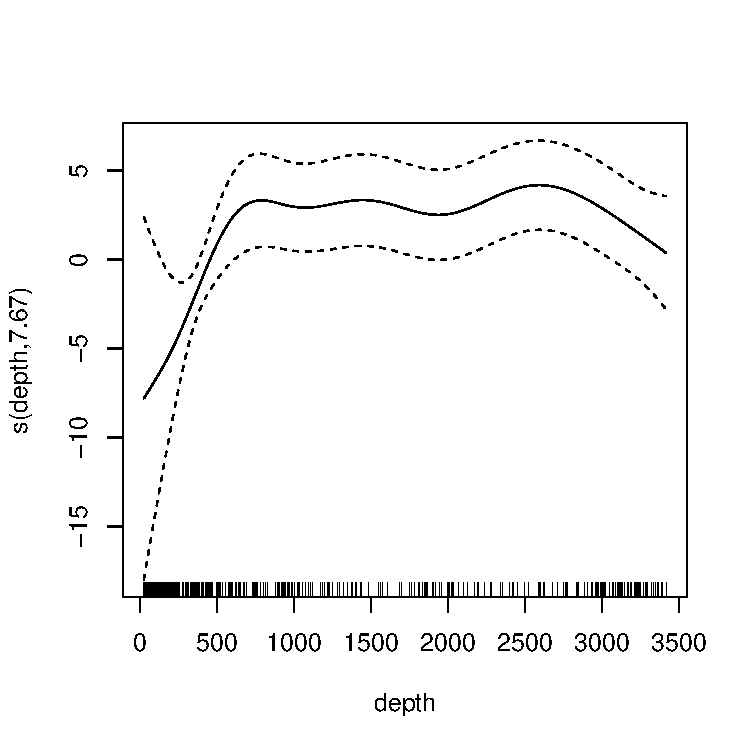
\includegraphics[width=\textwidth]{figs/fit-depth-gam}
  \end{center}
\end{figure}

\newpage

\begin{figure}[h!]
  \caption{Plot of coefficient of variation map for the model with smooths of both depth and location. Uncertainty was estimated using the variance propagation method of \cite{WILLIAMS:2011in}. As might be expected, there is high uncertainty where there is low sampling effort (Fig. \ref{dolphin-eda}).}
  \label{cv-plot}
  \begin{center}
    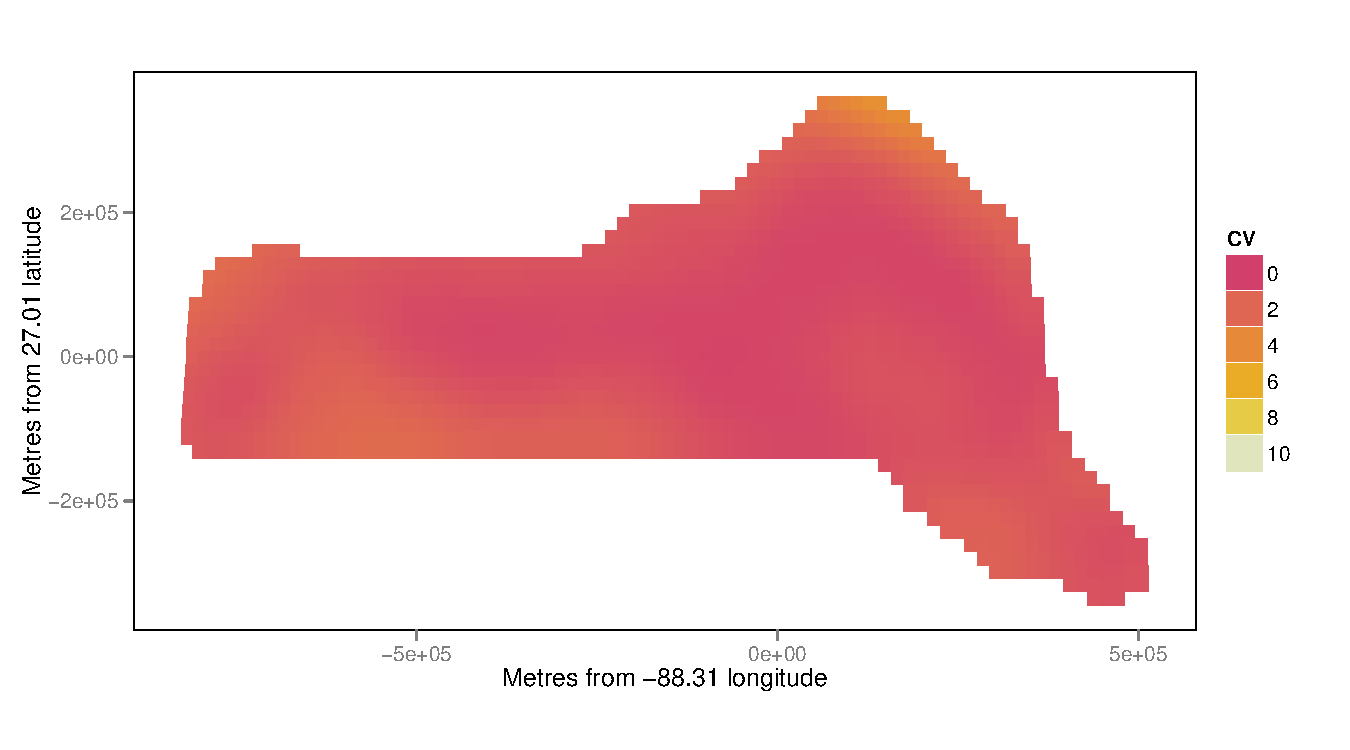
\includegraphics[width=\textwidth]{figs/cvplot-varprop}
  \end{center}
\end{figure}

\newpage

\begin{figure}[h!]
  \caption{Flow diagram showing the modelling process for creating a density surface model.}
  \label{flow}
  \begin{center}
    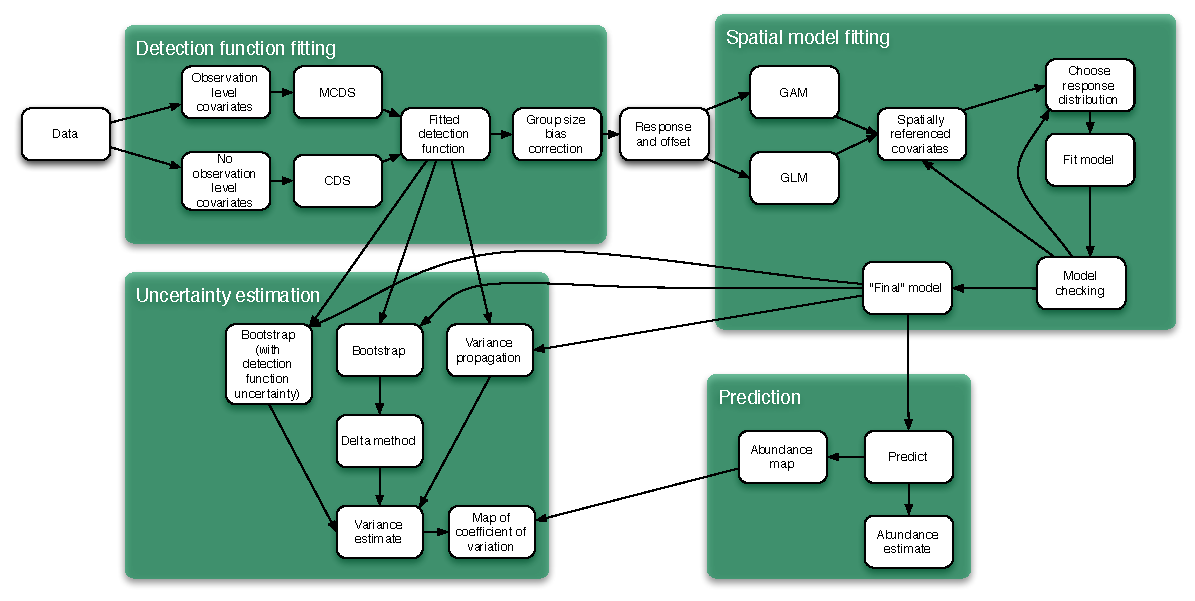
\includegraphics[height=\textheight]{figs/flowdiagram-reduced}
  \end{center}
\end{figure}

\newpage

%\begin{figure}[h!]
%  \caption{Example of model diagnostics for the model which included both location and depth covariates for the dolphin data when a quasi-Poisson response distribution was specified. From top left clockwise:  1) normal Q-Q plot showing a problematic fit (the ``elbow'' in the points), 2) plot of (deviance) residuals against predicted values highlighting outliers and LOESS smooth (\cite{Cleveland:1979vd}) through the point overlaid, 3) a smooth of location fitted to the residuals showing some pattern left in the data and 4) the autocorrelogram. }
%  \label{dsm-check}
%  \begin{center}
%    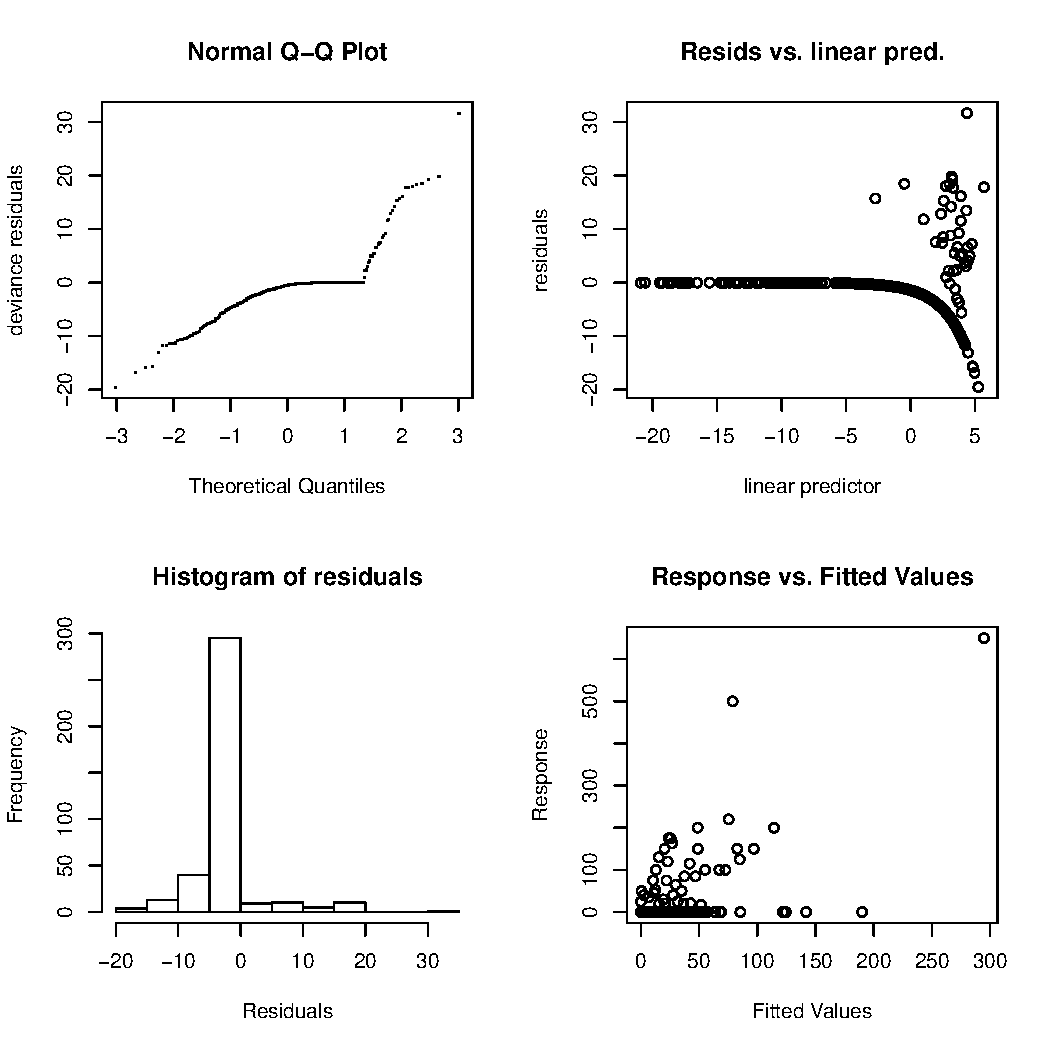
\includegraphics[width=\textwidth]{figs/dsm-check}
%  \end{center}
%\end{figure}


\end{document}
